

hwloc usually manipulates processing units and memory but it can also discover I/O devices and report their locality as well. This is useful for placing I/O intensive applications on cores near the I/O devices they use, or for gathering information about all platform components.

 \hypertarget{a00384_iodevices_enabling}{}\section{Enabling and requirements}\label{a00384_iodevices_enabling}
I/O discovery is disabled by default (except in lstopo) for performance reasons. It can be enabled by changing the filtering of I/O object types to {\ttfamily \hyperlink{a00193_gga9a5a1f0140cd1952544477833733195ba63fd24954e18c83ff7eae9588759adb5}{H\+W\+L\+O\+C\+\_\+\+T\+Y\+P\+E\+\_\+\+F\+I\+L\+T\+E\+R\+\_\+\+K\+E\+E\+P\+\_\+\+I\+M\+P\+O\+R\+T\+A\+NT}} or {\ttfamily \hyperlink{a00193_gga9a5a1f0140cd1952544477833733195bafda7b59e6810dfe778d8f9a4cc1e350e}{H\+W\+L\+O\+C\+\_\+\+T\+Y\+P\+E\+\_\+\+F\+I\+L\+T\+E\+R\+\_\+\+K\+E\+E\+P\+\_\+\+A\+LL}} before loading the topology, for instance with {\ttfamily \hyperlink{a00193_ga0ab38705357bc1203abe829da8a12ad3}{hwloc\+\_\+topology\+\_\+set\+\_\+io\+\_\+types\+\_\+filter()}}.

Note that I/O discovery requires significant help from the operating system. The pciaccess library (the development package is usually {\ttfamily libpciaccess-\/devel} or {\ttfamily libpciaccess-\/dev}) is needed to fully detect P\+CI devices and bridges/switches. On Linux, P\+CI discovery may still be performed even if {\ttfamily libpciaccess} cannot be used. But it misses P\+CI device names. Moreover, some operating systems require privileges for probing P\+CI devices, see \hyperlink{a00394_faq_privileged}{Does hwloc require privileged access?} for details.

The actual locality of I/O devices is only currently detected on Linux. Other operating system will just report I/O devices as being attached to the topology root object.

 \hypertarget{a00384_iodevices_objects}{}\section{I/\+O objects}\label{a00384_iodevices_objects}
When I/O discovery is enabled and supported, some additional objects are added to the topology. The corresponding I/O object types are\+: 
\begin{DoxyItemize}
\item {\ttfamily \hyperlink{a00184_ggacd37bb612667dc437d66bfb175a8dc55a51e7280240fd9f25589cbbe538bdb075}{H\+W\+L\+O\+C\+\_\+\+O\+B\+J\+\_\+\+O\+S\+\_\+\+D\+E\+V\+I\+CE}} describes an operating-\/system-\/specific handle such as the {\itshape sda} drive or the {\itshape eth0} network interface. See \hyperlink{a00384_iodevices_osdev}{OS devices}. 
\item {\ttfamily \hyperlink{a00184_ggacd37bb612667dc437d66bfb175a8dc55a5d8117a54df1fbd3606ab19e42cb0ea9}{H\+W\+L\+O\+C\+\_\+\+O\+B\+J\+\_\+\+P\+C\+I\+\_\+\+D\+E\+V\+I\+CE}} and {\ttfamily \hyperlink{a00184_ggacd37bb612667dc437d66bfb175a8dc55a6825f10895fea60aca7a6ba9fe273db0}{H\+W\+L\+O\+C\+\_\+\+O\+B\+J\+\_\+\+B\+R\+I\+D\+GE}} build up a P\+CI hierarchy made of bridges (that may be actually be switches) and devices. See \hyperlink{a00384_iodevices_pci}{P\+CI devices and bridges}. 
\end{DoxyItemize}Any of these types may be filtered individually with {\ttfamily \hyperlink{a00193_gad894e70f15f8d4aada7be8d1aba38b7e}{hwloc\+\_\+topology\+\_\+set\+\_\+type\+\_\+filter()}}.

hwloc tries to attach these new objects to normal objects (usually N\+U\+MA nodes) to match their actual physical location. For instance, if a I/O hub (or root complex) is physically connected to a package, the corresponding hwloc bridge object (and its P\+CI bridges and devices children) is inserted as a child of the corresponding hwloc Package object. {\bfseries These children are not in the normal children list but rather in the I/\+O-\/specific children list.}

I/O objects also have neither C\+PU sets nor node sets (N\+U\+LL pointers) because they are not directly usable by the user applications for binding. Moreover I/O hierarchies may be highly complex (asymmetric trees of bridges). So I/O objects are placed in specific levels with custom depths. Their lists may still be traversed with regular helpers such as \hyperlink{a00187_ga759e88eaf5a230ad283e9d4c42486735}{hwloc\+\_\+get\+\_\+next\+\_\+obj\+\_\+by\+\_\+type()}. However, hwloc offers some dedicated helpers such as \hyperlink{a00204_ga66470dabce9db19a57c5940a909d0baa}{hwloc\+\_\+get\+\_\+next\+\_\+pcidev()} and \hyperlink{a00204_ga8b4584c8949e2c5f1c97ba7fe92b8145}{hwloc\+\_\+get\+\_\+next\+\_\+osdev()} for convenience (see \hyperlink{a00204}{Finding I/O objects}).

 \hypertarget{a00384_iodevices_osdev}{}\section{O\+S devices}\label{a00384_iodevices_osdev}
Although each P\+CI device is uniquely identified by its bus ID (e.\+g. 0000\+:01\+:02.\+3), a user-\/space application can hardly find out which P\+CI device it is actually using. Applications rather use software handles (such as the {\itshape eth0} network interface, the {\itshape sda} hard drive, or the {\itshape mlx4\+\_\+0} Open\+Fabrics H\+CA). Therefore hwloc tries to add software devices ({\ttfamily \hyperlink{a00184_ggacd37bb612667dc437d66bfb175a8dc55a51e7280240fd9f25589cbbe538bdb075}{H\+W\+L\+O\+C\+\_\+\+O\+B\+J\+\_\+\+O\+S\+\_\+\+D\+E\+V\+I\+CE}}, also known as OS devices).

OS devices may be attached below P\+CI devices, but they may also be attached directly to normal objects. Indeed some OS devices are not related to P\+CI. For instance, N\+V\+D\+I\+MM block devices (such as {\itshape pmem0s} on Linux) are directly attached near their N\+U\+MA node (I/O child of the parent whose memory child is the N\+U\+MA node). Also, if hwloc could not discover P\+CI for some reason, P\+C\+I-\/related OS devices may also be attached directly to normal objects.

hwloc first tries to discover OS devices from the operating system, e.\+g. {\itshape eth0}, {\itshape sda} or {\itshape mlx4\+\_\+0}. However, this ability is currently only available on Linux for some classes of devices.

hwloc then tries to discover software devices through additional I/O components using external libraries. For instance proprietary graphics drivers do not expose any named OS device, but hwloc may still create one OS object per software handle when supported. For instance the {\ttfamily opencl} and {\ttfamily cuda} components may add some {\itshape opencl0d0} and {\itshape cuda0} OS device objects.

Here is a list of OS device objects commonly created by hwloc components when I/O discovery is enabled and supported.


\begin{DoxyItemize}
\item Hard disks or non-\/volatile memory devices (\hyperlink{a00184_gga64f5d539df299c97ae80ce53fc4b56c0a689b0488c3c0d08d116751c6b9cb8871}{H\+W\+L\+O\+C\+\_\+\+O\+B\+J\+\_\+\+O\+S\+D\+E\+V\+\_\+\+B\+L\+O\+CK}) 
\begin{DoxyItemize}
\item {\itshape sda} or {\itshape dax2.\+0} (Linux component) 
\end{DoxyItemize}
\item Network interfaces (\hyperlink{a00184_gga64f5d539df299c97ae80ce53fc4b56c0ab715d81155f771573c8682dffc65021b}{H\+W\+L\+O\+C\+\_\+\+O\+B\+J\+\_\+\+O\+S\+D\+E\+V\+\_\+\+N\+E\+T\+W\+O\+RK}) 
\begin{DoxyItemize}
\item {\itshape eth0}, {\itshape wlan0}, {\itshape ib0} (Linux component) 
\end{DoxyItemize}
\item Open\+Fabrics (Infini\+Band, Omni-\/\+Path, us\+N\+IC, etc) H\+C\+As (\hyperlink{a00184_gga64f5d539df299c97ae80ce53fc4b56c0a52157d03694fdae82dddd57ca8c973b6}{H\+W\+L\+O\+C\+\_\+\+O\+B\+J\+\_\+\+O\+S\+D\+E\+V\+\_\+\+O\+P\+E\+N\+F\+A\+B\+R\+I\+CS}) 
\begin{DoxyItemize}
\item {\itshape mlx5\+\_\+0}, {\itshape hfi1\+\_\+0}, {\itshape qib0}, {\itshape usnic\+\_\+0} (Linux component) 
\end{DoxyItemize}
\item G\+P\+Us (\hyperlink{a00184_gga64f5d539df299c97ae80ce53fc4b56c0aa3a09798ef2836abb236dc3a645ffc90}{H\+W\+L\+O\+C\+\_\+\+O\+B\+J\+\_\+\+O\+S\+D\+E\+V\+\_\+\+G\+PU}) 
\begin{DoxyItemize}
\item {\itshape rsmi0} for the first R\+S\+MI device (R\+S\+MI component, using the A\+MD R\+O\+Cm S\+MI library) 
\item {\itshape nvml0} for the first N\+V\+ML device (N\+V\+ML component, using the N\+V\+I\+D\+IA Management Library) 
\item {\itshape \+:0.\+0} for the first display (GL component, using the N\+V-\/\+C\+O\+N\+T\+R\+OL X extension library, N\+V\+Ctrl) 
\end{DoxyItemize}
\item Co-\/\+Processors (\hyperlink{a00184_gga64f5d539df299c97ae80ce53fc4b56c0a46f8927e1c3e137eaa86cc8f6861fb83}{H\+W\+L\+O\+C\+\_\+\+O\+B\+J\+\_\+\+O\+S\+D\+E\+V\+\_\+\+C\+O\+P\+R\+OC}) 
\begin{DoxyItemize}
\item {\itshape opencl0d0} for the first device of the first Open\+CL platform, {\itshape opencl1d3} for the fourth device of the second Open\+CL platform (Open\+CL component) 
\item {\itshape cuda0} for the first N\+V\+I\+D\+IA C\+U\+DA device (C\+U\+DA component, using the N\+V\+I\+D\+IA C\+U\+DA Library)  
\item D\+MA engine channel (\hyperlink{a00184_gga64f5d539df299c97ae80ce53fc4b56c0a827ad1643360711a8b6c6af671366791}{H\+W\+L\+O\+C\+\_\+\+O\+B\+J\+\_\+\+O\+S\+D\+E\+V\+\_\+\+D\+MA}) 
\begin{DoxyItemize}
\item {\itshape dma0chan0} (Linux component) when all OS devices are enabled (\hyperlink{a00193_gga9a5a1f0140cd1952544477833733195bafda7b59e6810dfe778d8f9a4cc1e350e}{H\+W\+L\+O\+C\+\_\+\+T\+Y\+P\+E\+\_\+\+F\+I\+L\+T\+E\+R\+\_\+\+K\+E\+E\+P\+\_\+\+A\+LL}) 
\end{DoxyItemize}
\end{DoxyItemize}

Note that some P\+CI devices may contain multiple software devices (see the example below).

See also \hyperlink{a00390}{Interoperability With Other Software} for managing these devices without considering them as hwloc objects.

 
\end{DoxyItemize}\hypertarget{a00384_iodevices_pci}{}\section{P\+C\+I devices and bridges}\label{a00384_iodevices_pci}
A P\+CI hierarchy is usually organized as follows\+: A hostbridge object ( {\ttfamily \hyperlink{a00184_ggacd37bb612667dc437d66bfb175a8dc55a6825f10895fea60aca7a6ba9fe273db0}{H\+W\+L\+O\+C\+\_\+\+O\+B\+J\+\_\+\+B\+R\+I\+D\+GE}} object with upstream type {\itshape Host} and downstream type {\itshape P\+CI}) is attached below a normal object (usually the entire machine or a N\+U\+MA node). There may be multiple hostbridges in the machine, attached to different places, but all P\+CI devices are below one of them (unless the Bridge object type is filtered-\/out).

Each hostbridge contains one or several children, either other bridges (usually P\+CI to P\+CI switches) or P\+CI devices ({\ttfamily \hyperlink{a00184_ggacd37bb612667dc437d66bfb175a8dc55a5d8117a54df1fbd3606ab19e42cb0ea9}{H\+W\+L\+O\+C\+\_\+\+O\+B\+J\+\_\+\+P\+C\+I\+\_\+\+D\+E\+V\+I\+CE}}). The number of bridges between the hostbridge and a P\+CI device depends on the machine.

 \hypertarget{a00384_iodevices_consult}{}\section{Consulting I/\+O devices and binding}\label{a00384_iodevices_consult}
I/O devices may be consulted by traversing the topology manually (with usual routines such as \hyperlink{a00187_ga6f414dd80a2b943967a0ac92da3181a2}{hwloc\+\_\+get\+\_\+obj\+\_\+by\+\_\+type()}) or by using dedicated helpers (such as \hyperlink{a00204_gacdbaf0db98872e224b7883a84bfb0455}{hwloc\+\_\+get\+\_\+pcidev\+\_\+by\+\_\+busid()}, see \hyperlink{a00204}{Finding I/O objects}).

I/O objects do not actually contain any locality information because their C\+PU sets and node sets are N\+U\+LL. Their locality must be retrieved by walking up the object tree (through the {\ttfamily parent} link) until a non-\/\+I/O object is found (see \hyperlink{a00204_gaf139bb61375178e90cc3f1835b452ab6}{hwloc\+\_\+get\+\_\+non\+\_\+io\+\_\+ancestor\+\_\+obj()}). This normal object should have non-\/\+N\+U\+LL C\+PU sets and node sets which describe the processing units and memory that are immediately close to the I/O device. For instance the path from a OS device to its locality may go across a P\+CI device parent, one or several bridges, up to a Package node with the same locality.

Command-\/line tools are also aware of I/O devices. lstopo displays the interesting ones by default (passing {\ttfamily -\/-\/no-\/io} disables it).

hwloc-\/calc and hwloc-\/bind may manipulate I/O devices specified by P\+CI bus ID or by OS device name. 
\begin{DoxyItemize}
\item {\ttfamily pci=0000\+:02\+:03.\+0} is replaced by the set of C\+P\+Us that are close to the P\+CI device whose bus ID is given.  
\item {\ttfamily os=eth0} is replaced by C\+P\+Us that are close to the I/O device whose software handle is called {\ttfamily eth0}.  
\end{DoxyItemize}This enables easy binding of I/\+O-\/intensive applications near the device they use.

 \hypertarget{a00384_iodevices_examples}{}\section{Examples}\label{a00384_iodevices_examples}
The following picture shows a dual-\/package dual-\/core host whose P\+CI bus is connected to the first package and N\+U\+MA node.

 
\begin{DoxyImageNoCaption}
  \mbox{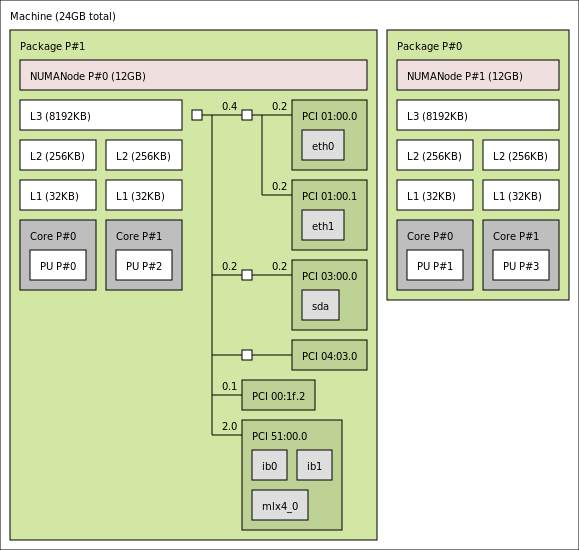
\includegraphics[width=\textwidth]{devel09-pci.png}}
\end{DoxyImageNoCaption}


Six interesting P\+CI devices were discovered. However, hwloc found some corresponding software devices ({\itshape eth0}, {\itshape eth1}, {\itshape sda}, {\itshape mlx4\+\_\+0}, {\itshape ib0}, and {\itshape ib1}) for only four of these physical devices. The other ones ({\itshape P\+CI 102b\+:0532} and {\itshape P\+CI 8086\+:3a20}) are an unused I\+DE controller (no disk attached) and a graphic card (no corresponding software device reported to the user by the operating system).

On the contrary, it should be noted that three different software devices were found for the last P\+CI device ({\itshape P\+CI 15b3\+:634a}). Indeed this Open\+Fabrics H\+CA P\+CI device object contains one one Open\+Fabrics software device ({\itshape mlx4\+\_\+0}) and two virtual network interface software devices ({\itshape ib0} and {\itshape ib1}).

Here is the corresponding textual output\+:

\begin{DoxyVerb}Machine (24GB total)
  Package L#0
    NUMANode L#0 (P#0 12GB)
    L3 L#0 (8192KB)
      L2 L#0 (256KB) + L1 L#0 (32KB) + Core L#0 + PU L#0 (P#0)
      L2 L#1 (256KB) + L1 L#1 (32KB) + Core L#1 + PU L#1 (P#2)
    HostBridge
      PCIBridge
        PCI 01:00.0 (Ethernet)
          Net "eth0"
        PCI 01:00.1 (Ethernet)
          Net "eth1"
      PCIBridge
        PCI 03:00.0 (RAID)
          Block "sda"
      PCIBridge
        PCI 04:03.0 (VGA)
      PCI 00:1f.2 (IDE)
      PCI 51:00.0 (InfiniBand)
        Net "ib0"
        Net "ib1"
        Net "mlx4_0"
  Package L#1
    NUMANode L#1 (P#1 12GB)
    L3 L#1 (8192KB)
      L2 L#2 (256KB) + L1 L#2 (32KB) + Core L#2 + PU L#2 (P#1)
      L2 L#3 (256KB) + L1 L#3 (32KB) + Core L#3 + PU L#3 (P#3)
\end{DoxyVerb}
 